% Paths relative to this package root; requires graphicx.
\begin{figure}[tbp]
\centering
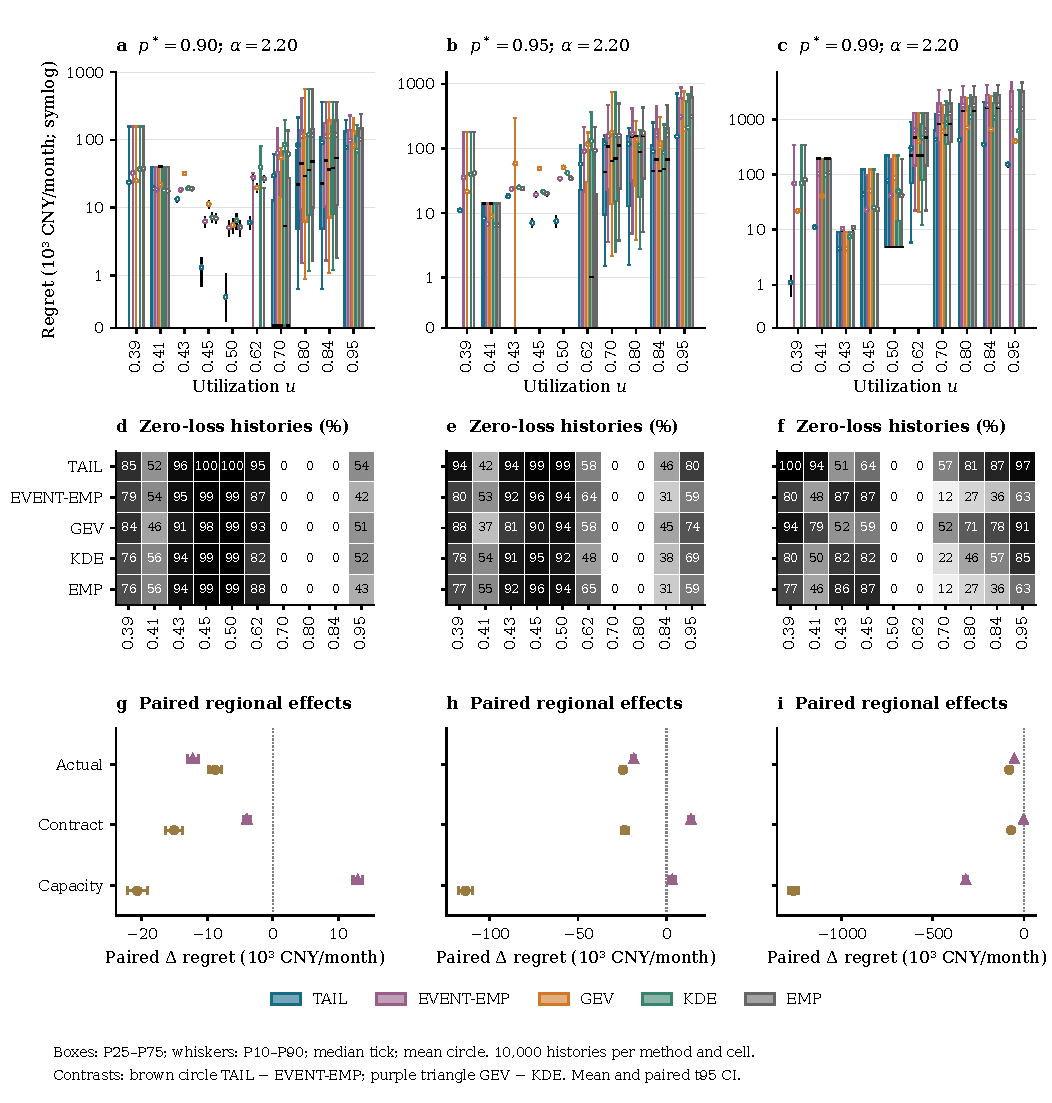
\includegraphics[width=\linewidth]{figures/FigureS1.pdf}
\caption{High-contract-quantile stress experiment at alpha = 2.20, comprising 10,000 histories, five methods, three target quantiles, and ten utilization cells per target quantile (1,500,000 decisions). Columns correspond to target quantiles 0.90, 0.95, and 0.99. (a--c) Cellwise regret distributions: boxes span P25--P75, whiskers P10--P90, black ticks denote medians, and open circles denote means; black intervals at means are pointwise 95\% Student t intervals (9,999 degrees of freedom). The symlog ordinate retains zero, is linear below one thousand CNY per month, and logarithmic above it; ranges vary by column. (d--f) Percentages of exactly zero regret, with the same grayscale mapping from 0 to 100 in all panels. Printed values are rounded to whole percentages; a printed 100 need not imply every history has zero regret. (g--i) Same-information paired regional mean differences: TAIL minus EVENT-EMP (circles) and GEV minus KDE (triangles). Cells are equally weighted within history and oracle region before differences are formed; intervals are paired t95 intervals. Negative values favour the first method. Data were reconstructed from saved fits without refitting or new simulation.}
\label{fig:final-figures1}
\end{figure}

\begin{figure}[tbp]
\centering
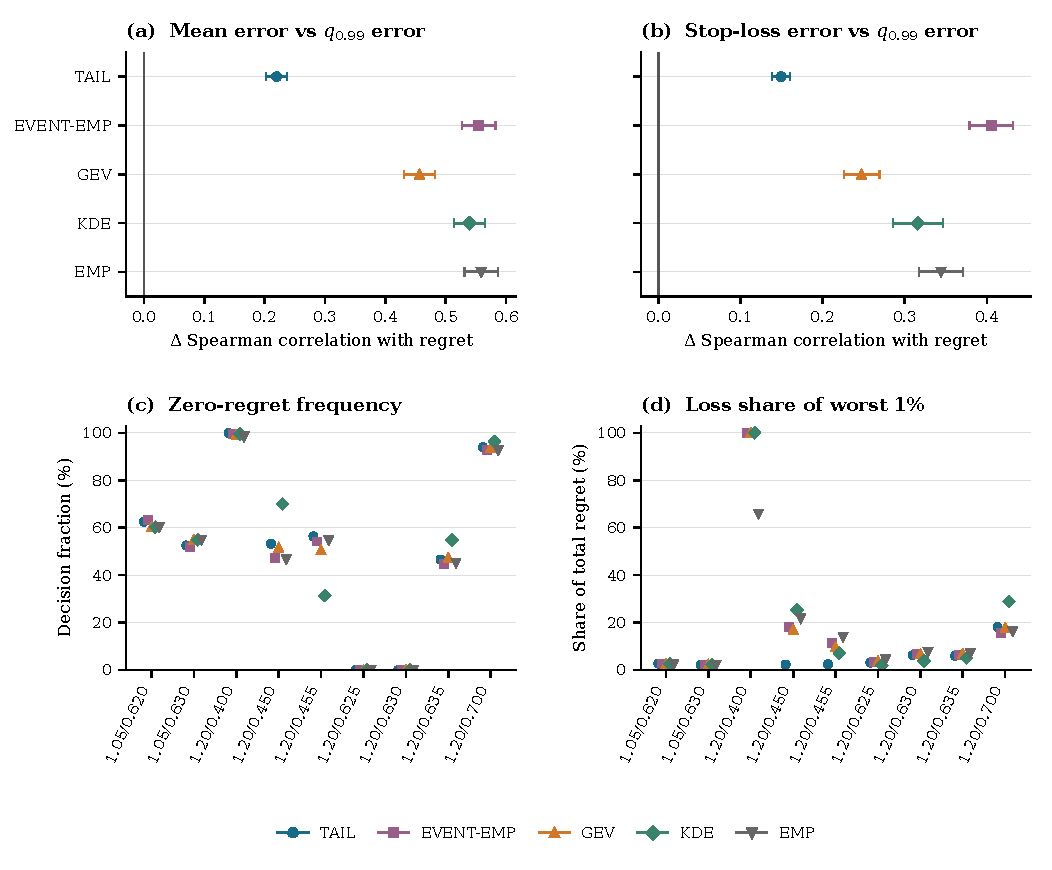
\includegraphics[width=\linewidth]{figures/FigureS2.pdf}
\caption{Functional-error associations and loss concentration. (a,b) Within-method differences between the Spearman correlation of regret with absolute mean or stop-loss relative error and its correlation with absolute $q_{0.99}$ relative error. Error and regret quantities are first averaged over nine cells within each of 10,000 histories. Intervals are the supplied simultaneous max-$|T|$ 95\% intervals for the family of ten correlation differences, based on 2,000 paired-history bootstrap resamples. They are not pointwise intervals. (c) Zero-regret frequency and (d) the share of aggregate regret accounted for by the worst 1\% of decisions within each method--cell sample. The lower panels are descriptive summaries from 10,000 histories per method and cell. Offset, unconnected points distinguish methods at discrete tariff cells; the positions do not form a continuous tariff response.}
\label{fig:final-figures2}
\end{figure}

\begin{figure}[tbp]
\centering
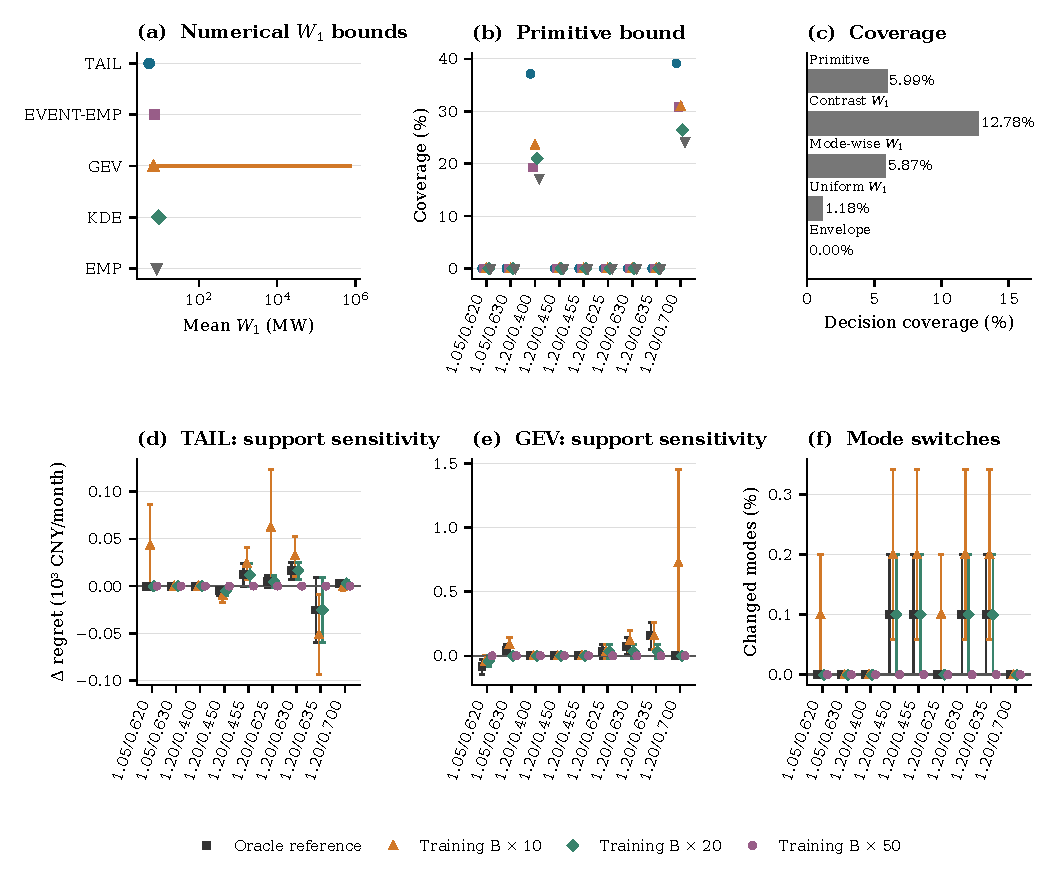
\includegraphics[width=\linewidth]{figures/FigureS3.pdf}
\caption{\textbf{Numerical distribution-to-decision bounds and
fitting-support sensitivity.}
\textbf{(a)} Mean $W_1$ point estimates and CDF-based numerical
lower and upper bounds over 10,000 fitted laws per method; the
logarithmic axis retains the loose GEV upper bound.
\textbf{(b)} Cellwise coverage of the primitive numerical
sufficient-condition check by predictive method.
\textbf{(c)} Overall coverage of the Primitive,
contrast-Wasserstein, mode-wise pairwise-Wasserstein,
uniform-Wasserstein, and coarse distributional-envelope checks over
450,000 primary decisions. The first four use the same numerical
full-action solver allowance. The contrast-Wasserstein and mode-wise
pairwise-Wasserstein checks differ in whether the common distributional
perturbation is bounded directly for each tariff contrast or after
separate mode-value bounds.
\textbf{(d,e)} Paired mean regret changes for TAIL and GEV under
alternative fitted-support rules relative to the primary
specification.
\textbf{(f)} Percentage of TAIL tariff-mode decisions that change
under each support rule. Error bars in (d--f) are one paired Monte
Carlo standard error over the first 1,000 primary histories.
Training-derived support rules use multipliers 10, 20, and 50;
Oracle reference denotes the diagnostic bound $10q_{0.999}$.
Point estimates in (a), the CDF-based bounds, and the solver
allowances are numerical rather than interval-certified quantities.}
\label{fig:final-figures3}
\end{figure}

\begin{figure}[tbp]
\centering
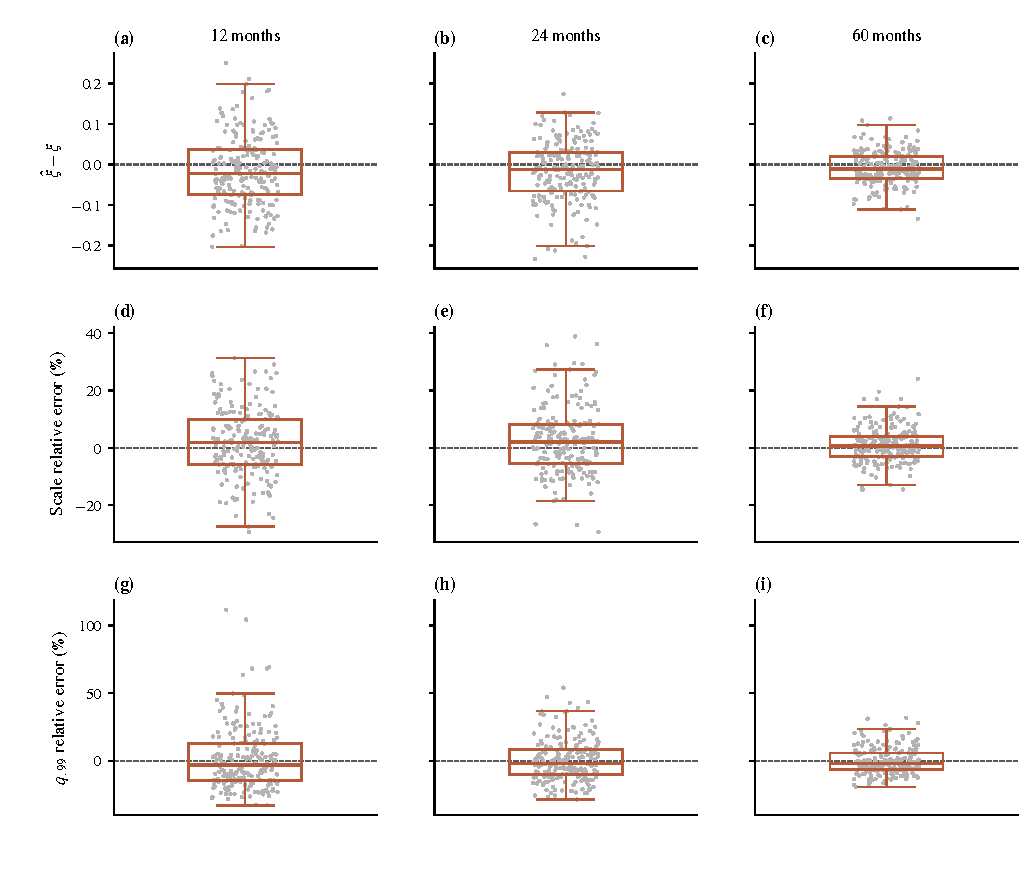
\includegraphics[width=\linewidth]{figures/FigureS4.pdf}
\caption{Parameter-recovery experiment. Columns show training
lengths of 12, 24, and 60 months; rows show GPD shape error, relative
scale error, and relative $q_{0.99}$ error. Each panel displays all
200 histories as grey points, with median, interquartile box, and
1.5-IQR whiskers. These are distribution summaries, not confidence
intervals; the recovery experiment is separate from the primary
analysis.}
\label{fig:final-figures4}
\end{figure}

\begin{figure}[tbp]
\centering
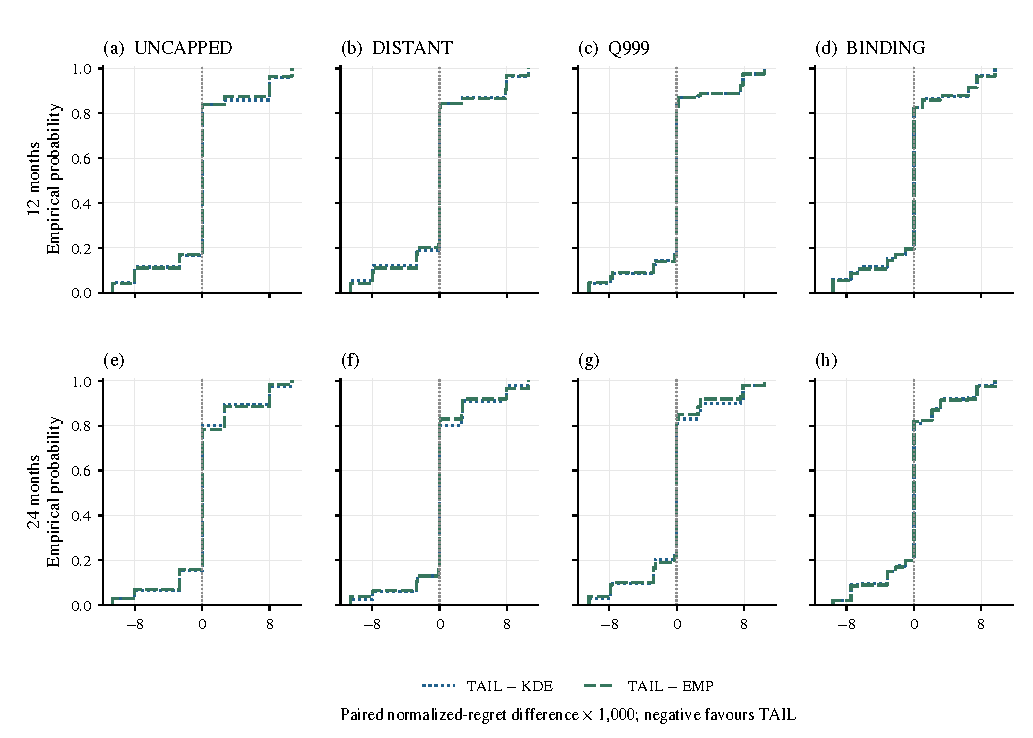
\includegraphics[width=\linewidth]{figures/FigureS5.pdf}
\caption{Physical clipping sensitivity. Columns show the four frozen
clipping regimes and rows show 12 or 24 training months. Each ECDF
contains 200 paired history differences in normalized regret times
1,000; negative values favour TAIL. The full data range is shown, and
the interquartile range is zero in all 16 groups. This descriptive
robustness experiment is separate from the primary analysis.}
\label{fig:final-figures5}
\end{figure}

\begin{figure}[tbp]
\centering
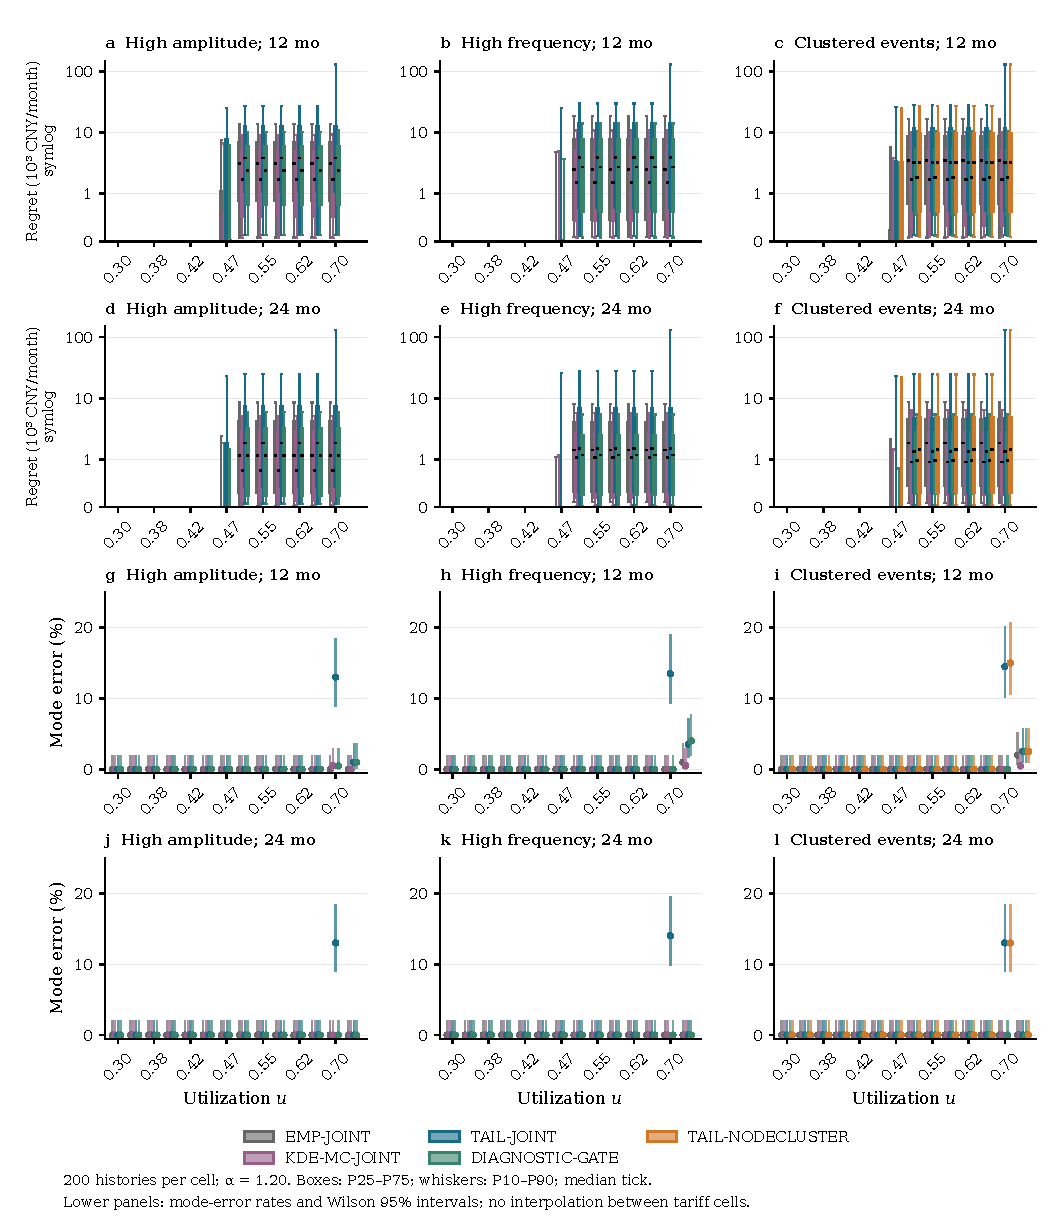
\includegraphics[width=0.94\linewidth]{figures/FigureS6.pdf}
\caption{Physical-pipeline experiments at alpha = 1.20 using 200
paired histories per method, training length, and tariff cell
(72,800 decisions). Columns represent high amplitude, high frequency,
and clustered events. (a--f) Regret distributions at all 14 utilization
cells for training lengths of 12 and 24 months: boxes span P25--P75,
whiskers span P10--P90, and black ticks denote medians. The symlog
ordinate retains zero and is linear below one thousand CNY per month.
Outlying histories beyond the whiskers are not drawn individually;
these are distribution summaries, not confidence intervals. (g--l)
Mode-error proportions and pointwise Wilson 95\% intervals at the
same cells. Points are offset within each cell to separate methods and
are not interpolated between cells. TAIL-NODECLUSTER applies only to
the clustered-event scenario.}
\label{fig:final-figures6}
\end{figure}

\begin{figure}[tbp]
\centering
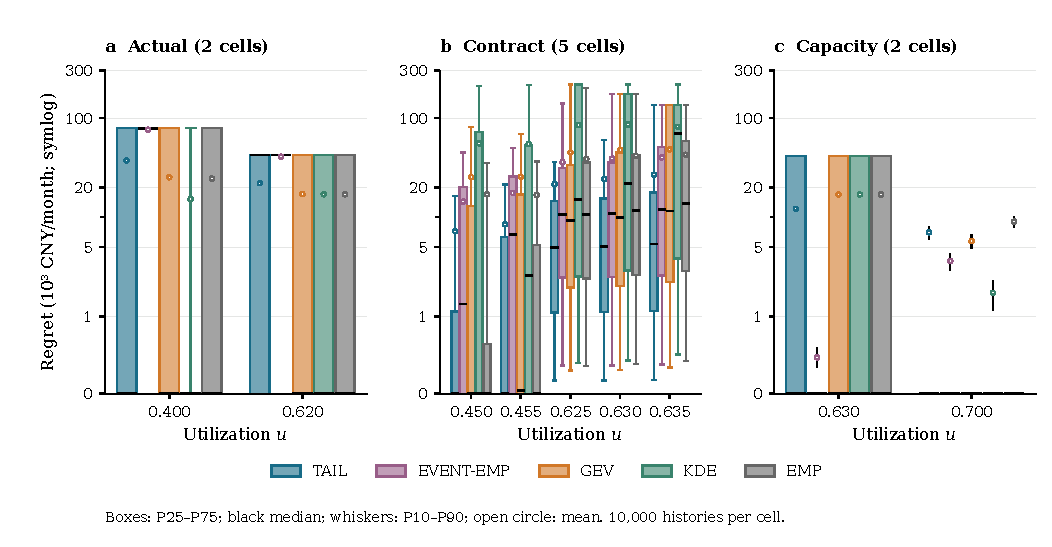
\includegraphics[width=\linewidth]{figures/FigureS7.pdf}
\caption{Cellwise regret distributions under the negative-binomial--Weibull challenge, with 10,000 histories per method and cell. Panels group the two actual, five contract, and two capacity oracle cells; labels give utilization and cells are equally spaced. Filled boxes span P25--P75, black ticks denote medians, whiskers span P10--P90, and open circles denote means. Black intervals at means use the formal pointwise normal 95\% approximation, mean plus or minus 1.96 standard errors. The symlog ordinate is linear below one thousand CNY per month and logarithmic above it. Histories outside the displayed quantile ranges are not drawn individually. Quantile ranges describe history variability and are distinct from uncertainty in the mean.}
\label{fig:final-figures7}
\end{figure}

\begin{figure}[tbp]
\centering
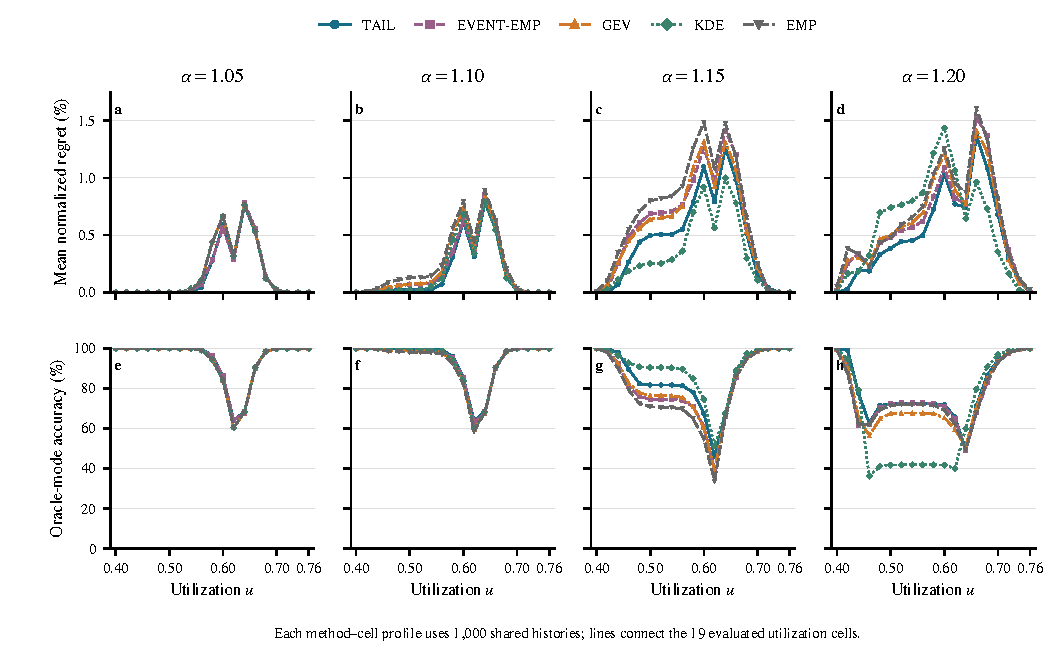
\includegraphics[width=\linewidth]{figures/FigureS8.pdf}
\caption{Complete five-method profiles over the final nonnegative, no-artificial-upper crossed tariff grid. Panels (a--d) show mean normalized full-action regret, $R/V_F^*$, and panels (e--h) show oracle-mode accuracy, for $\alpha=1.05$, 1.10, 1.15, and 1.20. Each panel covers the 19 evaluated utilization values; each method--cell estimate uses 1,000 shared histories, giving 380,000 decisions in total. Lines connect discrete evaluated cells for visual comparison and do not represent interpolation. The profiles are descriptive; no confidence intervals are shown and no invariant within-region ranking is asserted. TAIL and EVENT--EMP use event-level information; GEV, KDE, and EMP use monthly maxima.}
\label{fig:crossed-grid-all-methods}
\end{figure}


